\chapter{Resolving a Conducting Conformation of CFTR Using Free Energy Calculations}
\label{chap:opening}
\chapquote{You wanna fight?} {- Doctor Zachary Picker. Layperson. (personal communication)}
\setcounter{figure}{0}
\renewcommand{\thefigure}{\arabic{chapter}.\arabic{figure}}


\section*{\centering Abstract} 
The misfunction of the CFTR gene causes Cystic Fibrosis. This protein conducts both chloride and bicarbonate. Understanding how CFTR conducts ions is critical to ongoing drug discovery efforts to treat Cystic Fibrosis. Existing structures of CFTR raise unresolved qustions as to how CFTR conducts ions as they exhibit a constriction smaller than the ions themselves. This indicates that there must be some level of conformational change for ions to pass through this structure. Here we present innovative simulation techniques combining principal component analysis of 8 microseconds of protein simulations and new advances in free energy calculations to resolve the full conduction pathway in human CFTR. We also propose experimental single ion channel electrophysiology techniques to experimetnally test whether this conformation is physiologically important.  

The presented study differs in an important way from existing studies which explore protein conformational landscape. Existing studies have previously investigated the conformational space \textit{between} solved protein conformations. The presented study demonstrates that with careful application of modelling it  is now possible to go \textit{beyond} the conformational neighbourhood of existing protein structures.

The findings of this study demonstrate that computational power and protein forcefields are now sufficiently developed to take the advances of the cryo-EM ``resolution revolution" and elucidate even more of the protein conformational landscape. This heralds a new era of computational structural biolgoy and biophysics.


\section{Introduction}

Ion channels are critical clinical targets. Their regulation of cellular membrane potential makes them attractive targets for many lcinical therapies. The mechanism and conditions under which they open and close is a closely studied topic due to the ability of small molecule drugs to regulate this transition and the pathology that a misfuncitonal channel can cause, either from mutation or environmental changes. Perhaps the most well-known channelopathie is the misfunction of the anion channel, the Cystic Fibrosis Transmembrane conudtance Regulator (CFTR) which causes Cystic Fibrosis (CF) \cite{riordan1989,gadsby2006}. 

Various mutations may cause this ion channel to misfunction but the advent of new modulators heralds a new era in the treatment of this life-limiting disease. Due to the importance of the conductance of this channel in disease pathology, a molecular understanding behind the basis of its conductivity will inform the rational design of novel therapeutics to better patient outcomes. Unfortunately, current protein structures of this protein are insufficiently dilated in order to conducta nions, leaving unresolved questions behind the basis fo its conductivity. 

The cahnnel exhibits a slectivity filter which must be both narrow enough to partially dehydrate chloride and also large enough to allow the passage of large anions such as bicarbonate and glutathione \cite{}. 

\subsection{The outer pore in the Cryo-EM structure of phosphorylated human CFTR is not sufficiently open to conduct anions}

\section{Results}


\subsection{Long Simulations Reveal Motions which Dilate the Pore}
4 simulations were run of WT-CFTR of at least 2 microseconds each, for a total of 8.2 $\mu s$ of sampling. In post processing, the motions of the transmembrane helices were analysed using Principal Component Anlaysis which revelaed large motions in TM1 and TM6 which appeared as though they dilated the pore. 

\begin{figure}
	\label{PCA_motions}
	\begin{center}
		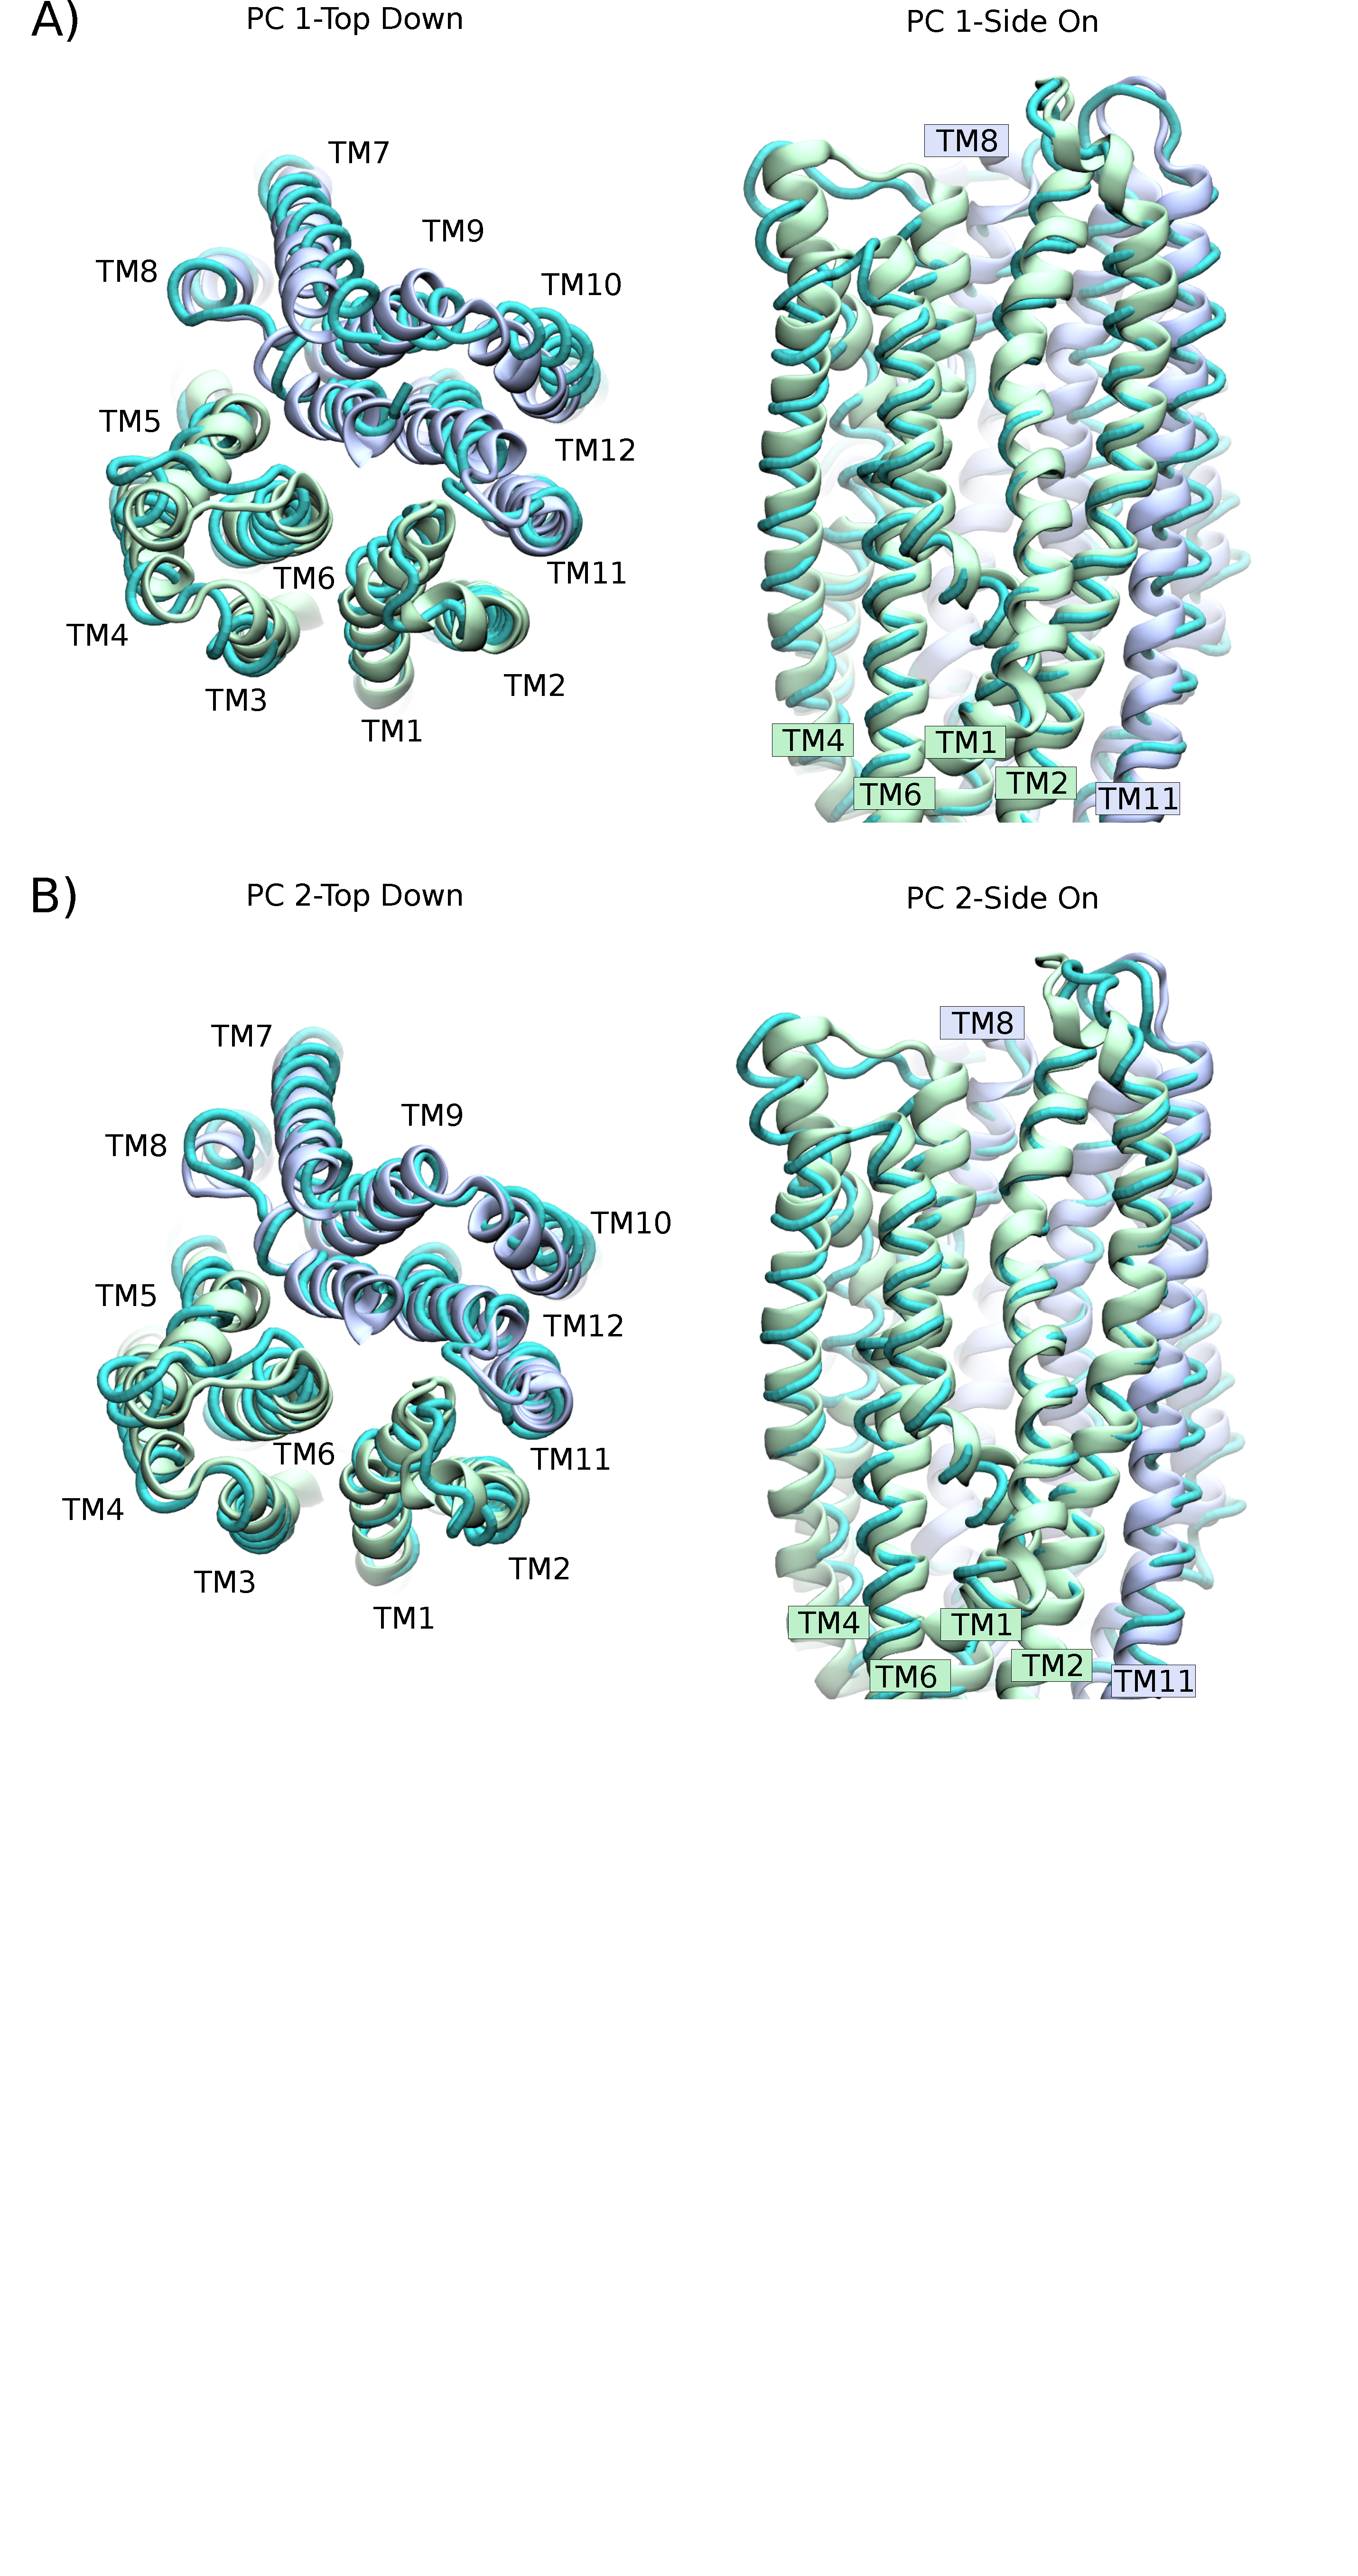
\includegraphics[width=1\textwidth]{figures/opening/pca_motions.pdf}
	\end{center}
	\captionsetup{singlelinecheck = false, justification=raggedright}
	\caption[Principal Component Analysis Reveals Large Motions in CFTR Transmembrane Helices] {\textbf{Principal Component Analysis Reveals Large Motions in CFTR Transmembrane Helices}}{A) Visualisation of the results of principal component analysis from 4 independent simulations, comprising 8.2 $\mu s$ of unbiased MD sampling. Motions along the first two principal component vectors were found to capture 38\% of the variation in the simulation and were used in further analysis. B) Visualisation of the first principal component vector (PC1). Note the motion in TMs 1, 6 and 8 C) Visualisation of the second principal component vector (PC2). Note the motions in TMs 1 and 6 but in directions orthogonal to PC1. D) Visualiastion of the Dilated Open state which we will analyse in detail in subsequent sections. This was obtained by the linear combination of PC 1 and 2. } 
\end{figure}

The first two principal components were chosen for further analysis as these two together represented 38\% of the kinetic variance in the unbiased data.

\subsection{Using OPES-Metadynamics we can find a stable configuration With an Open Pore}
We used the principal components discussed in the previous section were used as collective variables to study the motion of the transmembrane helices. By employing multiple walker OPES metadynamics we constructed the free energy surface in figure \ref{summary_FES}.

\begin{figure}
	\label{summary_FES}
	\begin{center}
		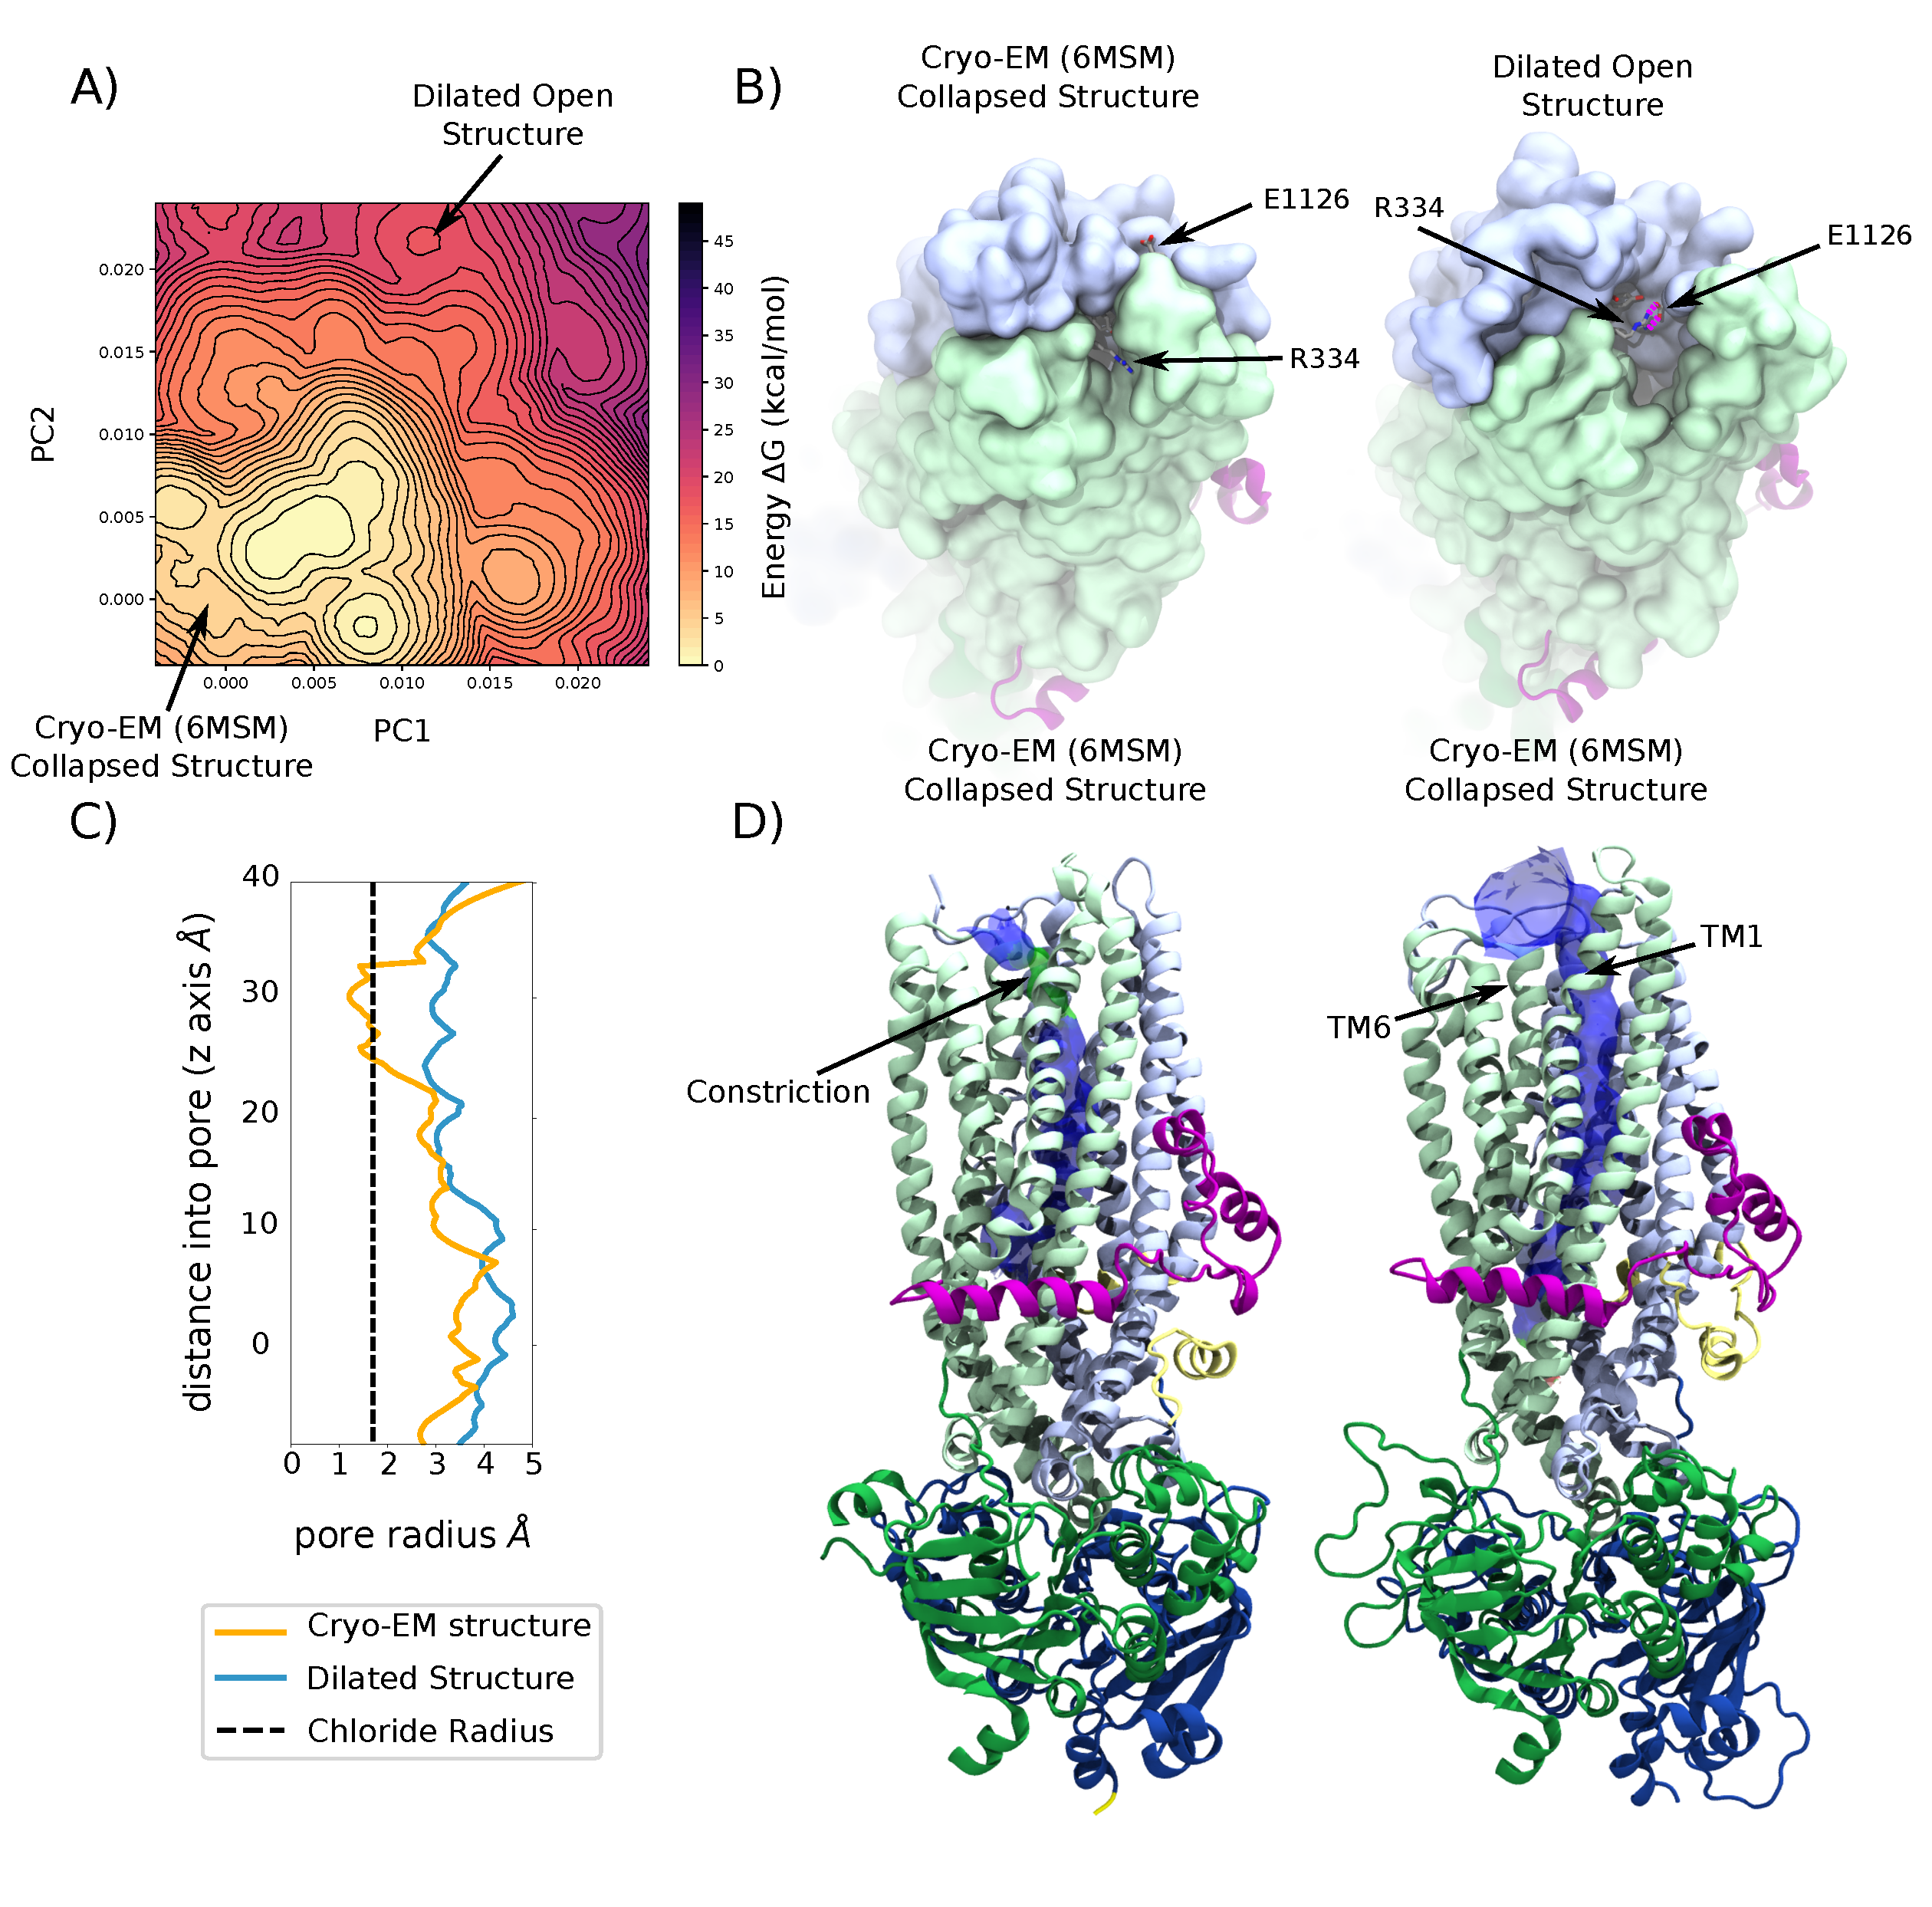
\includegraphics[width=1\textwidth]{figures/opening/summary_dilated_structure_1.pdf}
	\end{center}
	\captionsetup{singlelinecheck = false, justification=raggedright}
	\caption[Free Energy Calculations Discover a Dilated, Conformation of CFTR.] {\textbf{Free Energy Calculations Discover a Dilated, Conformation of CFTR.}}{A) B) C) D)}
\end{figure}

\subsection{This open conformation gives rise to a novel salt bridge}
In order to look for molecular interactions which might stabilise this open conformation, we inspected the interactions between pairs of positive and negative amino acids. It was found that a link between R334 and  E1126 could form in this new open state but not in the cryo-EM structure (Figure \ref{salt_bridge_fig}). This was possible due to the motions of TM6 and TM1, allowing E1126 on ECL5 to come closer to TM6. We expect this new salt bridge to be an important determining factor in stabilising the conducting conformation of CFTR.  

\label{salt_bridge}

\begin{figure}
	\label{salt_bridge_fig}
	\begin{center}
		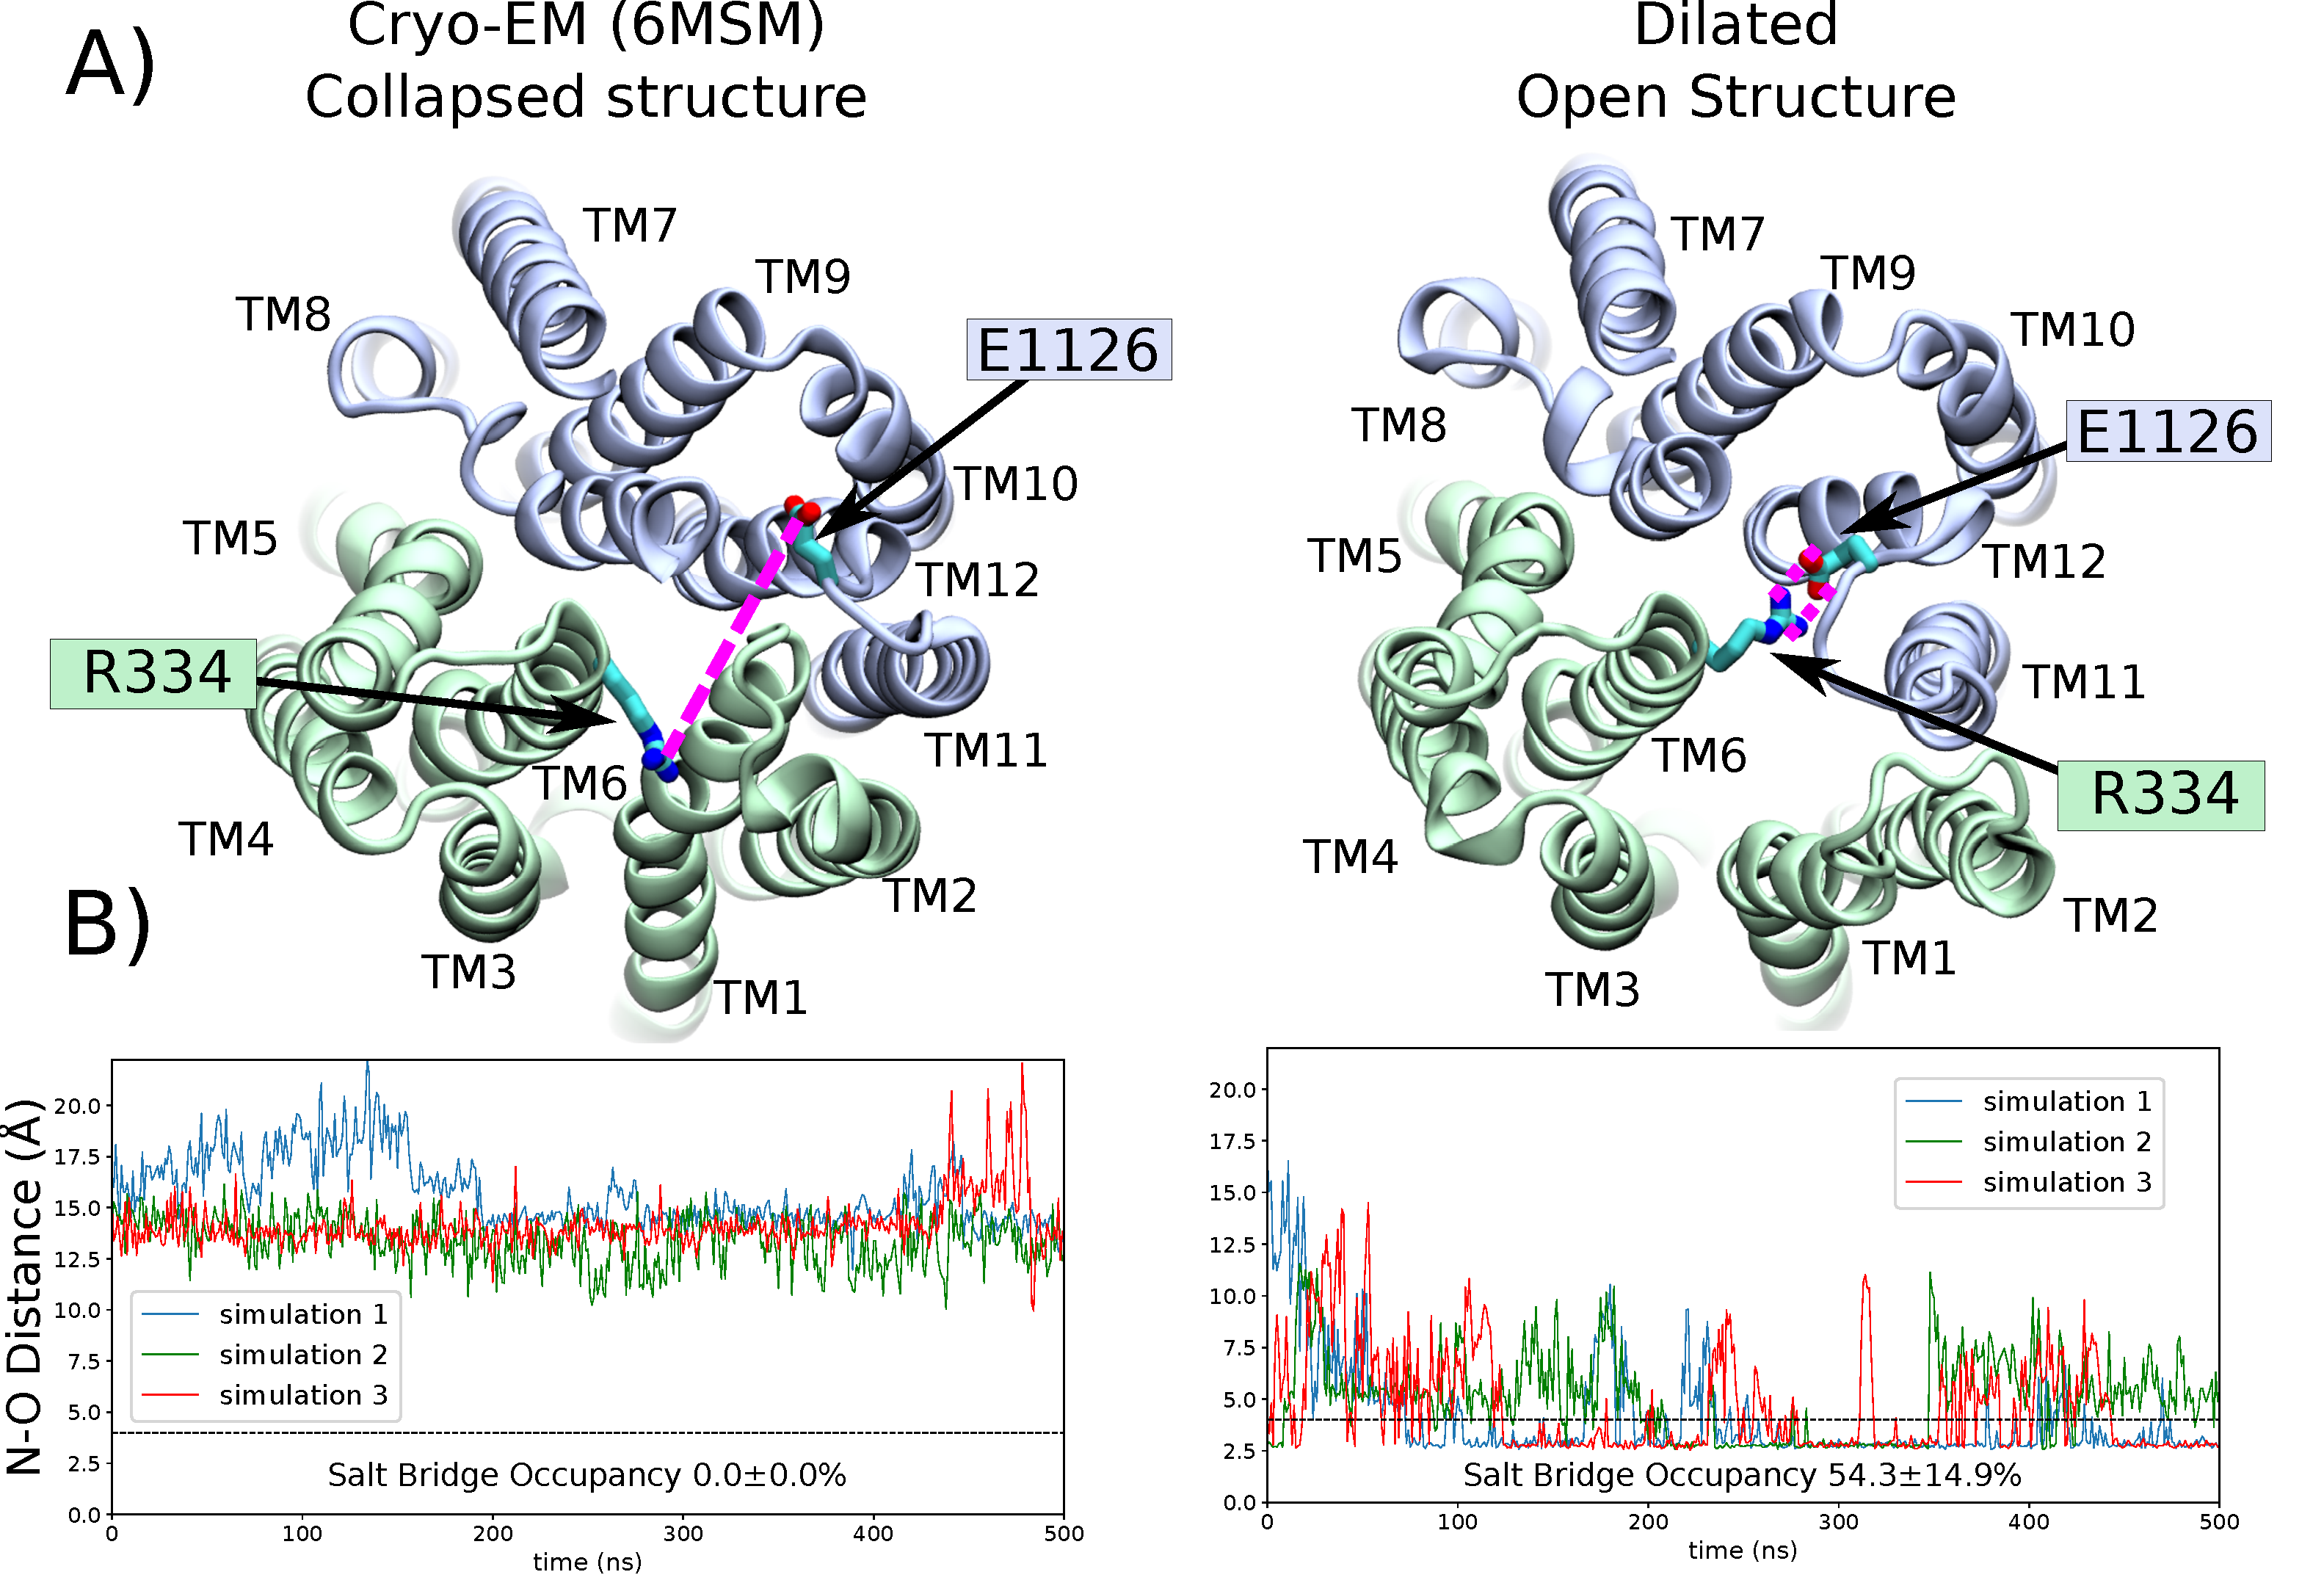
\includegraphics[width=1\textwidth]{figures/opening/salt_bridge_E1126_R334_figure.pdf}
	\end{center}
	\captionsetup{singlelinecheck = false, justification=raggedright}
	\caption[The Dilated Conformation of CFTR Gives Rise to the R334-E1126 Salt Bridge] {\textbf{The Dilated Conformation of CFTR Gives Rise to the R334-E1126 Salt Bridge}}{A) B) }
\end{figure}

\subsection{Proving the discovered conformation is capable of ion conduction with umbrella sampling}
In order to test the motion of the dilated structure to the passage of anions we employed umbrella sampling. After steering the channel into the opene state and then allowing it to equilibrate in that state for 80ns it was simulated for up to 500ns. This allowed us to test .

The free energy landscape of ions through the selectivity filter in the cryo-EM structure is not amenable to the movement of ions. We obtained a sizeable barrier of 9.7kcal/mol to the passage of ions, demonstrating that without dilation this structure will not allow ions to pass. By contrast, the dilated conformation which we discovered through metadynamics shows only a small free energy barrier of only 2.5 kcal/mol for both chloride and the larger bicarbonate. 

This small barrier roughly corresponds to what we would expect to be overcome by the natural 100mV polarisation of epithelial cells. Furhtermore, the remarkably similar profiles for both bicarbonate and chloride are in agreement with the energy landscape we would expect from a weakly selective channel like CFTR.

\begin{figure}
	\label{US_anions}
	\begin{center}
		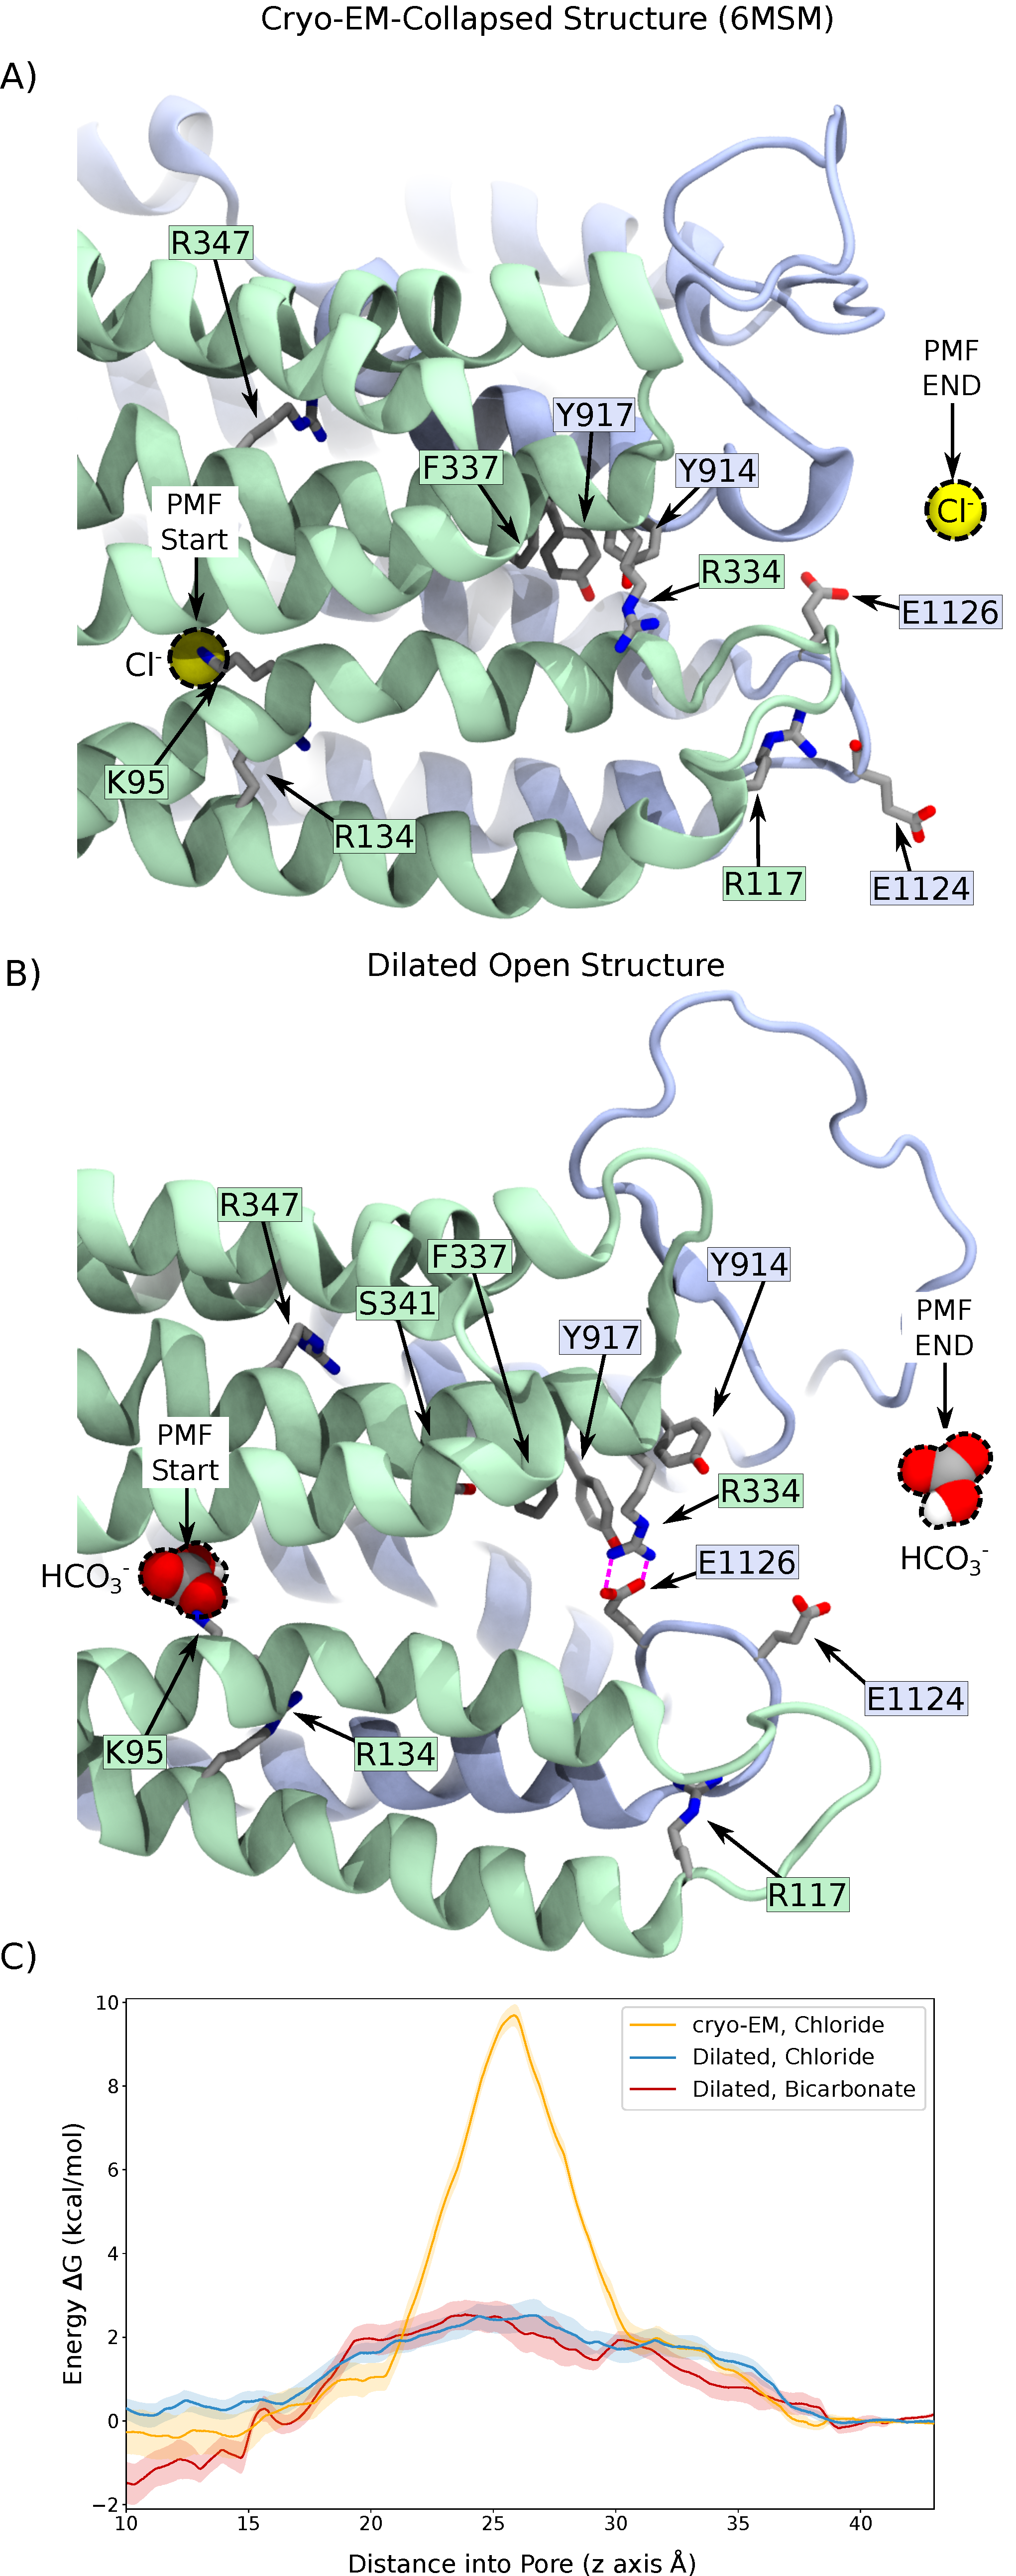
\includegraphics[width=0.6\textwidth]{figures/opening/pmf_fig_1_combined.pdf}
	\end{center}
	\captionsetup{singlelinecheck = false, justification=raggedright}
	\caption[The Dilated Conformation of CFTR is Capable of Conducting Anions] {\textbf{The Dilated Conformation of CFTR is Capable of Conducting Anions}}{A) B) C) D)}
\end{figure}



\subsection{This open state can be used to study disease causing mutations in the outer pore such as R334W}
Mutagenesis studies of the R334 amino acid noticed that many different mutations appear to result in ephys readings which would indicate a loss of function, including mutation to lysine (K) which seems surprising \cite{ge2004, gong2004, linsdell2021}. One of the more common disease causing missense mutations is R334W. This motivated the use of umbrella sampling to test the energy landscape of the chloride permeation pathway in the presence of this mutation. 


\begin{figure}
	\label{R334_pmf}
	\begin{center}
		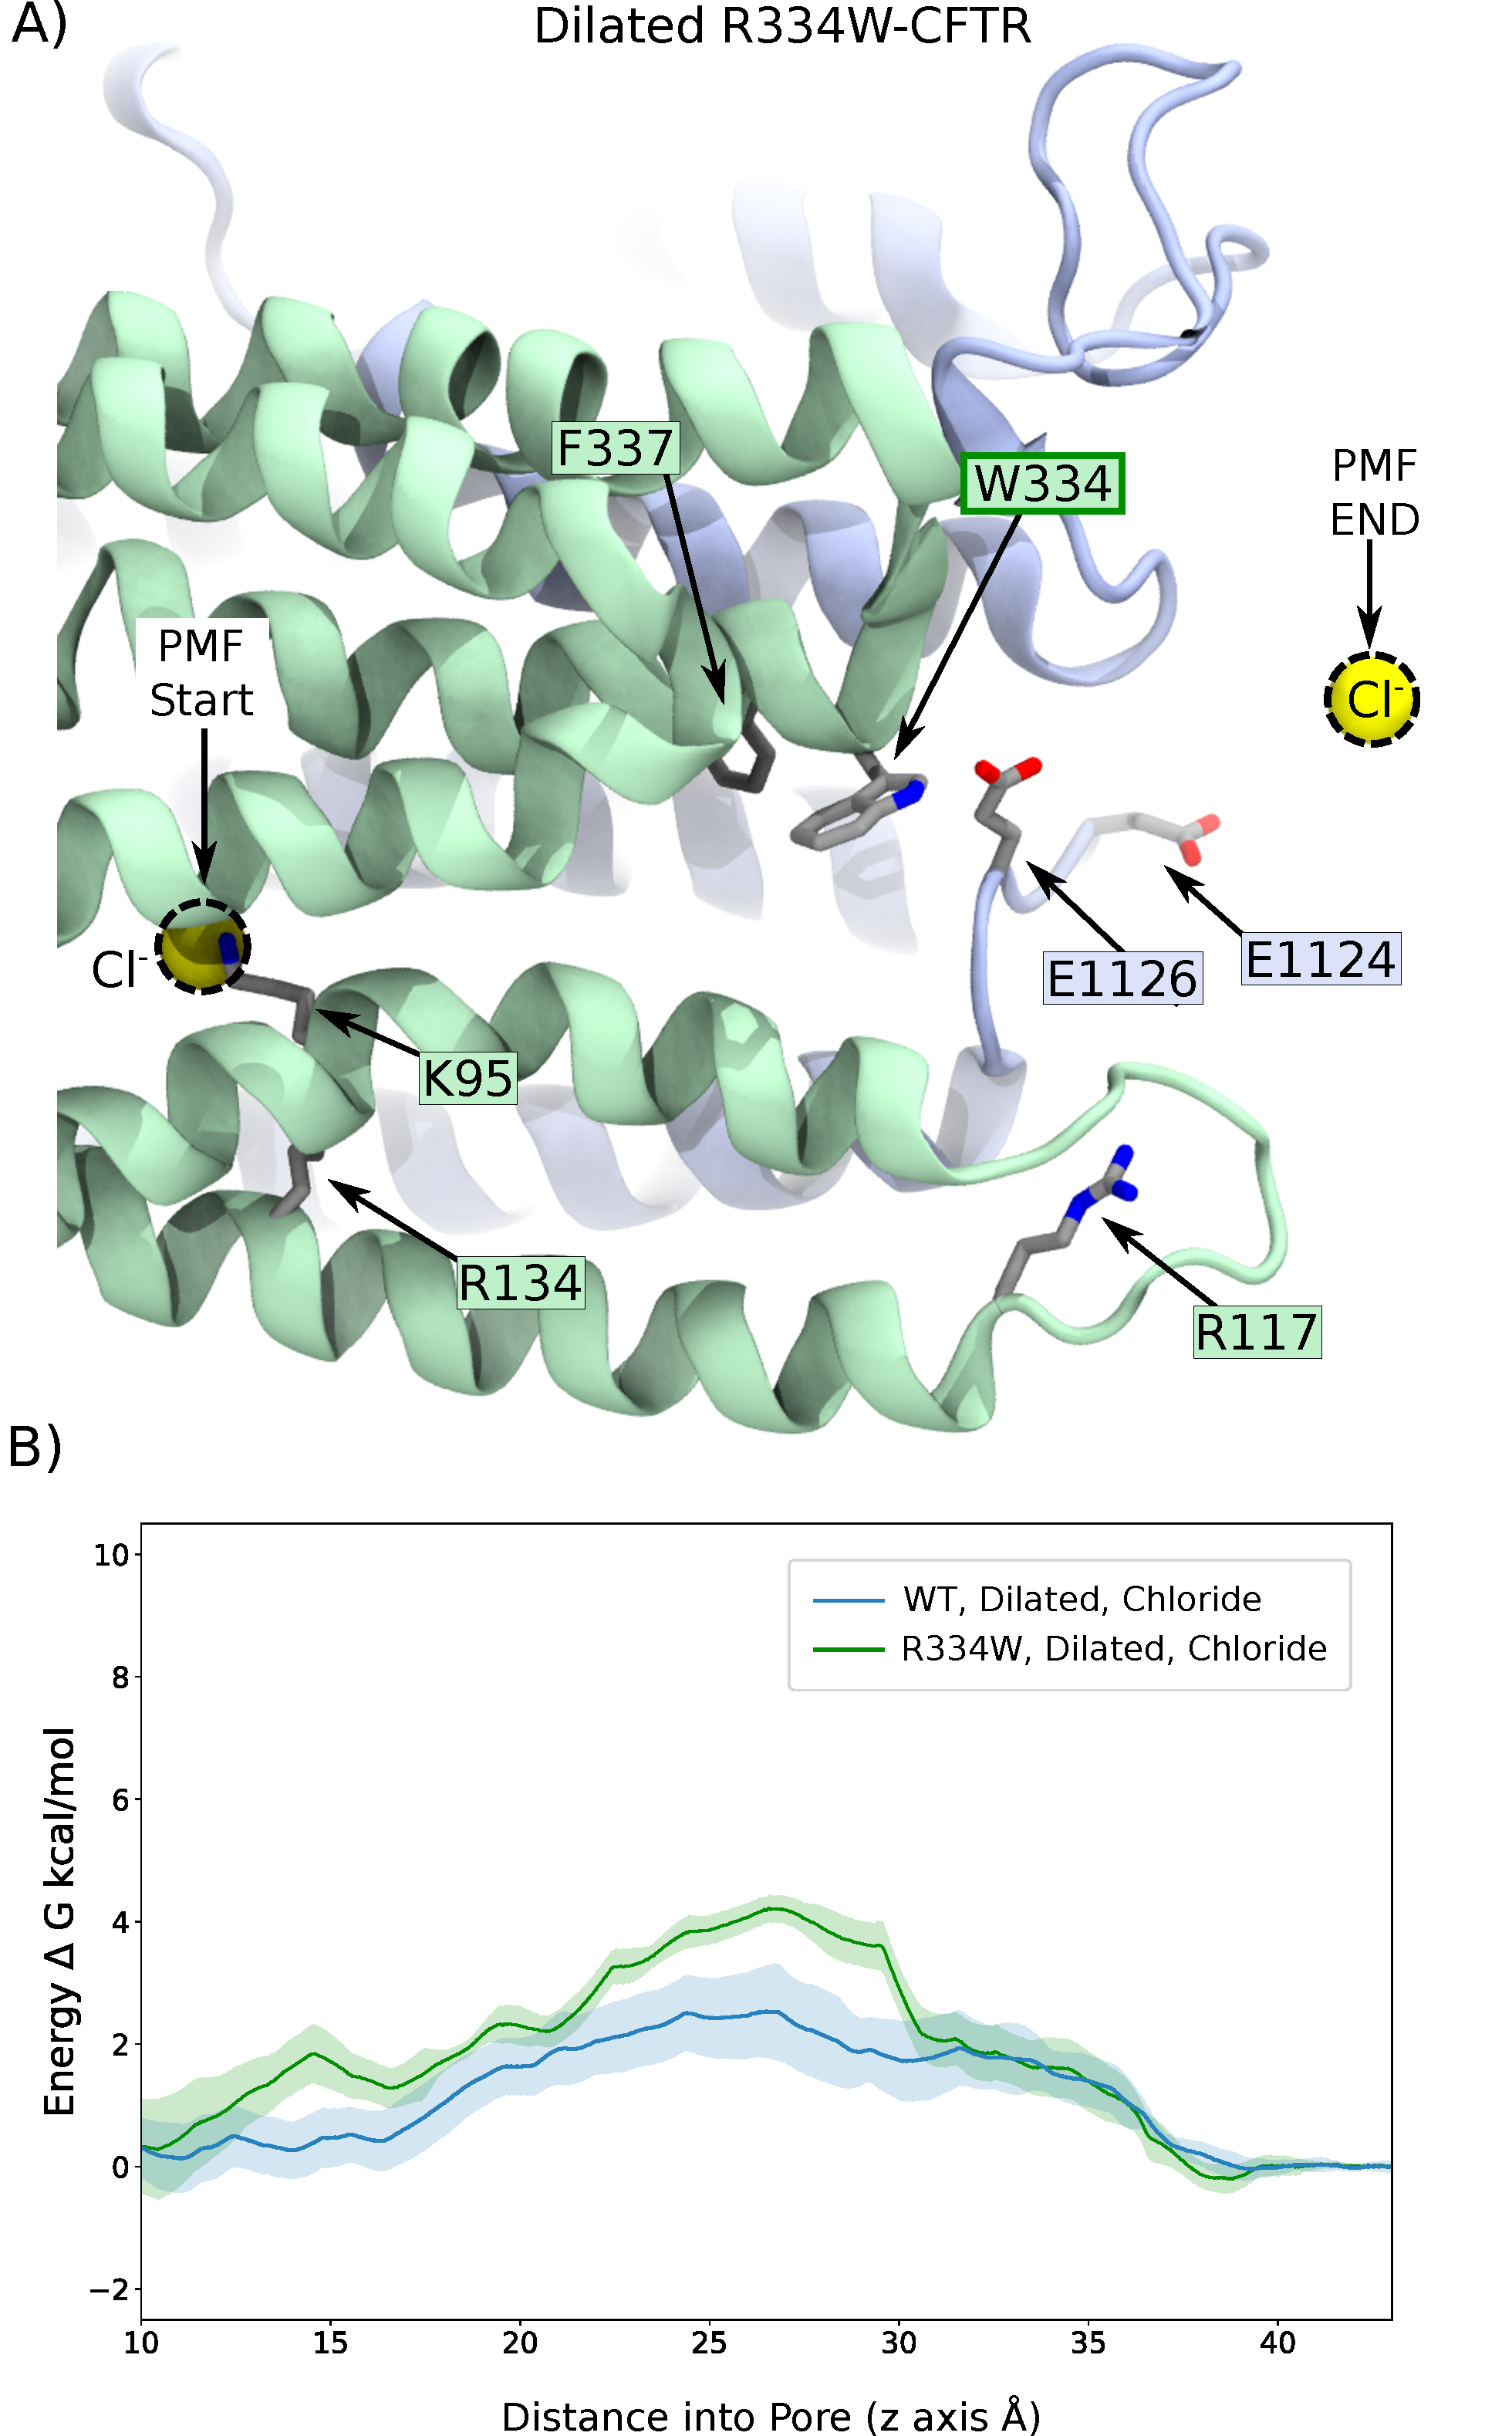
\includegraphics[width=0.6\textwidth]{figures/opening/R334W_pmf_combined.pdf}
	\end{center}
	\captionsetup{singlelinecheck = false, justification=raggedright}
	\caption[R334W Inhibits the Conduction of Anions] {\textbf{R334W inhibits the Conduction of Anions}}{A) B) C) D)}
\end{figure}

The energy landscape shows a clear barrier to chloride conductnace, even in the open structure, .

\section{Discussion}

The present study diverges in an important way from existing \textit{in silico} investigations of protein conformational changes. Past studies have focussed on recreating intermediate free energy landscapes between \textit{known} endpoints \cite{lev2020, bergh2021}. Such approaches are critical to the development of molecular techniques in order to understand the energetics and kinetics of protein systems. However, these studies are inherently limited to the availability of high quality experimental 3d structures. By using structures as a starting point we can explore the conformational space around a region to understand more about a protein system. This has been made possible by increasing the increasing accuracy of potein forcefields to reproduce structural ensembles \cite{huang2016} and considerable increases to computer power. The present study is akin to the development of an unsupervised vs. supervised machine learning algorithms. Each approach is powerful but has its own domain of applicability and drawbacks. 

I predict that as free energy calculations are increasingly used to study protein systems we will see a delineation between \textit{untargetted} and \textit{targetted} MD methods, similar to how we see a delineation between supervised and unsupervised machine learning techniques.

We can regard cryo-EM structures as points in the braoder free energy landscape of protein conformations. What we seek to do is build on these structural snapshots using simulations. Using unbiased MD we can explore a small slice of the local neighbourhood surrounding an experimentally determined atomic structure. Further, with the advent of free eneryg calculations to accelerate the slower degrees of freedom we can explore an even larger neighbourhood, giving a more complete picture of the molecular biophysics. 

\begin{figure}
	\label{Enhanced_sampling_framework}
	\begin{center}
		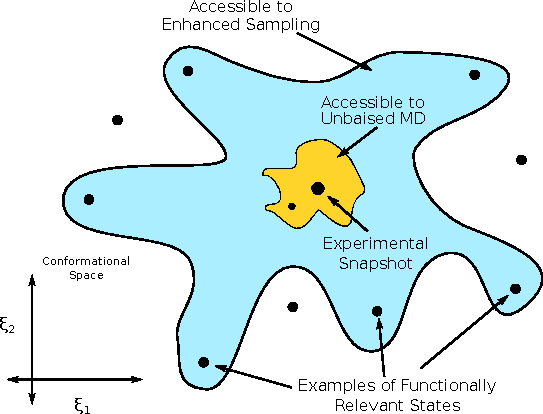
\includegraphics[width=0.6\textwidth]{figures/opening/MD_accessibility.pdf}
	\end{center}
	\captionsetup{singlelinecheck = false, justification=raggedright}
	\caption[Enhanced Sampling Allows Access to More Protein States] {\textbf{Enhanced Sampling Allows Access to More Protein States}}{The ``Resolution Revolution" in structural biolgy, fuelled by cryo-EM has lead to an era of structural abundance \cite{kuhlbrandt2014}. This means we have many structural snapshots of proteins with which to begin our study of their physical mechanisms. With unbiased MD simulations we can explore a small local neighbourhood surrounding these snapshots, shedding limited light on adjacent physilogically relevant funcational states. With Enhanced Sampling Techniques and Free energy calcuations we can access and study many more functional states. The more advanced these statistical techniques become the more functional states we will be able to access. These states might reveal drug binding pockets or the underlying mechanism behind the protein's function \cite{}.  . }
\end{figure}

What is perhaps remarkable about this study is just how well the results correspond with \textit{in vitro} biophysical experiments. The movements in TM1 and TM6 which dominate the PCA motions we accelerated are the kind of dilation we expected from biophysical experiments \cite{linsdell2016}. The distances from Y914 to L102 and . Additionally, the similar conductance profiles are the kind we expect from a weakly selective anion channel like CFTR. 

Surprisingly, the R334W mutation was determined not to alter the selectivity of CFTR \cite{sheppard1993}. This is an argument for a wider open pore at the R334 position, consistent with the findings of this study.

We should take note of some features which are lacking from our propsed open state which we expect of the fully open structure. Careful biophysical experiments discovered an interaction between the R117 and the carboxyl atom of E1124. This interaction was not present in our open state, nor was it well preserved in our unbaised simulations of the cryo-EM conformation. Similarly, the well characterised R104-E116 interaction is poorly preserved in both simulations. In our simulations we observed that these salt bridges were often broken (in the opened and unopened states) due to interactions with phosphate head groups in the phospholipid bilayer. Given the importance of different lipid species to regulation of CFTR such as cholesterol and sphingolipids, we expect that the zwitterionic POPC lipids used as a model membrane in this study do not fully reflect the native lipid environment of CFTR \cite{farinha2018, cottrill2020}. Recent studies have demonstrated an increasing need to study the bidirectional relationship between membrane composition and membrane protein regulation \cite{lin2022, kapoor2021, cui2020}. There are sadly few examples where membrane proteins have been characterised in both in both detergents and detergent micelles and nano discs revealed different side-chain conformations (however, the backbone was conserved) \cite{autzen2019, gao2016, cheng2015}. Hence, the state of the literature suggests that the salt bridges we mentioned earlier may in fact be regulated by the local environment of lipids around those specific sections of CFTR. Readers are encouraged to undertake studies to investigate the molecular fingerprint of the environment around CFTR.

The dilated structure we present has a significant motion in TM1 . This is  the kind of change we would expect from experiments studying the binding of WNK1. These studies demonstrate binding to TM1 favors the wide open conformation for the movement of bicarbonate ions \cite{kim2019}. 

As shown by the results in the present study, the difficulty in converging a free energy landscape with collective variables derived \textit {ab initio} from long classical MD simulations can be difficult as the CVs are very likely going to be suboptimal. Machine learning techniques, more sophisticated than the simple PCA algorithm used here would likely do a much better job of choosing quickly converging CVs \cite{}. 

The conformational changes investigated in this study occur within the lipid bilayer. This means that the kinetics and energetics of the transitions we have discovered will be highly dependent on the composition of lipids of the epithelium. It is well understood that the bilayer composition plays an important role in CFTR regulation and the clinical implications of this are an active area of research \cite{cui2020, cottrill2020}. It would therefore be an interesting study to repeat similar free energy calculations with different bilayer compositions to understand how they might regulate such conformational changes.

Understanding the open structure of CFTR has important implications for the drug discovery efforts to treat Cystic Fibrosis and sheds light on other important clinical questions. Specificlaly, selectivity of bicarbonate has been found to play an important role in pancreatic sufficiency of patients. The elucidation of basic CFTR function using simulations heralds an exciting new era of Cystic Fibrosis research. We are performing molecular medicine with atomic precision. 

The predictions of a stable salt bridge in section \ref{salt_bridge} fill a recent gap in the literature. The elegant study on the R117H mutation from Simon and Csnady's group \cite{simon2021}  discovered that a long standing conclusion that R117 made a connection with E1126 was incorrect and in fact R117 makes a stable hydrogen bond with E1124. This study did not closely investigate the role of E1126, observing that the E1126P mutant had slower closing kinetics but was unable to definitely explain why, suggesting that ECL6 might move slower in this mutation. This leaves the partner of E1126 unknown. One study investigating the blockage of CFTR by zinc postulated at an interaction between R334 and E1126 \cite{wang2016}. Here, the researchers tested the inhibition of chloride conduction in the presence of zinc in R334C-CFTR. They found strong evidence that R334C-CFTR was blocked by Zinc ions, as no current was recorded in the presence of zinc. Because zinc has a +2 charge they suspected that a nearby negative amino acid might might play a role in binding the zinc cation. Subsequent experiments They found that the mutant R334C/E1126A-CFTR was no longer inhibited by zinc ions. This is consistent with our findings that R334 and E1126 may indeed form a salt bridge, coming closer together in the conducting conformation compared to how far they are in the cryoEM structure.  

Previously it would have been very difficult to discover this interaction experimentally because R334 has plays such an important role in the conductance and selectivity of the channel. With the use of the atomic resolution offered by MD simulations we have been able to fill this gap in the experimental literature, demonstrating the power of \textit {in silico} methods for studying protein dynamics. We propose that single ion channel patch clamp experiments could demonstrate teh importance of teh E1126-R334 salt bridge to the open state of the channel. 

Similar to how this study was motivated by the lack of a structural picture of CFTR's conducting state, there are many other places in the proteome which would likely be amenable to a similar mode of investigation. For example, the important ABC transporter P-glycoprotein has been resolved in an outward facing occluded state, but the important outward facing conformation remains unimaged \cite{}. A similar technique to the one used here could likely resolve such a conformation \cite{kim2018a}.

\textit {in vitro} studies of the state dependent formation of the extracellular helices of the distances between  TM1, TM6, and TM12 indicated that in the closed state these helices are tightly bound together (as can be seen in the 6MSM structure) and in the open state they move apart \cite{negoda2018}. Additionally, similar studies of TM8 demonstrate that Y914 and Y917 are solvent exposed, pore lining helices, position 914 linked to position 102 and 334 when they were each replaced by cysteines. Interestingly, the distance in our proposed open structure is similar to that found in 6MSM, consistent with these experiments \cite{negoda2019}. 

Mutations at R334 also exhibit a gating defect, with infrequent transitions to the fully open state \cite{zhang2005a ,cui2013a, sheppard1993}. However, the specifics of the burst kinetics of this mutation are understudied, likely because of the low counductiviyt of the R334W-CFTR channel which makes electrophysiology experiments difficult. This reveals the niche for simuations, since we have atomic resolution into the dynamics of this channel, we can study the interacitons in the mutant where it might be hard to do experimentally. It is likely that an involved path Metadynamics or string method with swarms of trajectories approach might reveal the pathogenic gating defect present in this mutation. Construction of such a protocol could be used to investigate outher outer viestibutle gating class defects such as R117.

The simulations results we have found here would make us strongly expect a gating phenotype for an E1126 mutant to look like the R334C measuremnts found in \ref{zhang2005a}. This single ion channel study found infrequent transitions to the fully open state with frequent transitions to the transiently open state. This is consistent with the model we have proposed from our study here.

The work in this chapter suggests that computaitonal methods are now sufficiently developed such that creative application of MD simluations and free energy techniques can sehd light on the molecular mechanism of proteins. A limited but powerful example of this would be to further refine the methods applied in this chapter and then apply them to the partially collapsed structure of P-glycoprotein and dilate it in order to resolve the fully outward facing configuration.

\section{Conclusion}
With innovative application of free energy techniques we have been able to study an open, conducting conformation of CFTR. The conducting state of the channel has critical importance to drug discovery efforts for potentiators. If a small molecule drug could be developed to favor this state it would be a highly effective drug, as potentiators have demonstrated life changing clinical efficacy.

\section{Methods Details}
\subsection{System Composition}
At a basic level, methodology used in this chapter is largely consistent with the other studies in this thesis with some key differnces. The system was also constructed by embedding the extended CFTR model into a POPC membrane and then the whole these biomolecules were immersed in a neutralising 0.15 mol/L KCl solution. For all calculations in this chapter, except the initial unbiased calculations, the C-terminus was trunked at amino acid 1450 in order to make the simluation box smaller and save computer time.

\subsection{Unbiased MD }
The minimisation and equilibration steps for these simulations were largely carried out in the same way as for previous chapters. Our protein model was the extended CFTR model based on the 6MSM structure \cite{zhang2018} which we constructed in chapter \ref{chap:I37R}. The MD system was subjected to minimisation by steepest descent followed by restrained relaxation. This involved 10 kcal/mol $\AA^2$ harmonic restraints on all heavy protein atoms with restraints halved every 400 picoseconds. This relaxation was followed by up to 2.2 $\mu$s of unbiased molecular dynamics sampling.

\subsection {Principal Component and Choice of Collective Variable for OPES-Metadynamics}
In order to exclude large, fast motions like those from disordered loops, we limited our analysis to the following amino acids.

\begin{table}
	\label{red_alpha_carbons}
	\begin{center}
	%\begin{tabular} {| c | c | c | c | c | c | c | c | c | c | c | c | }  
	\resizebox{0.85\textwidth}{!}{%
	\begin{tabular} {| c | c | c | c | c | c | c | c | c | c | c | c | }  
		\hline
		\textbf{TM1}  $\uparrow$ & \textbf{TM2}  $\downarrow$ & \textbf{TM3}  $\uparrow$ & \textbf{TM4}   $\downarrow$& \textbf{TM5}  $\uparrow$ & \textbf{TM6}   $\downarrow$& \textbf{TM7}  $\uparrow$ & \textbf{TM8}   $\downarrow$& \textbf{TM9}   $\uparrow$& \textbf{TM10} $\downarrow$ & \textbf{TM11}  $\uparrow$ & \textbf{TM12}   $\downarrow$\\ \hline

                         & 113                      &  218 & 219 &                          &                          & 885 &                          &                           & 1013 &                            &                           \\ \hline
                         & 114                      &  217 & 220 &                          &                          & 884 &                          &                           & 1014 &                            &                           \\ \hline
                         & 115                      &  216 & 221 &                          &                          & 883 &                          &                           & 1015 &                            &                           \\ \hline
                         & 116                      &  215 & 222 &                          &                          & 882 &                          &                           & 1016 &                            &                           \\ \hline
                         & 117                      &  214 & 223 &                          &                          & 881 &                          &                           & 1017 &                            &                           \\ \hline
112                      & 118                      &  213 & 224 & 330                      &                          & 880 &                          &                           & 1018 &                            & 1124                      \\ \hline
111                      & 119                      &  212 & 225 & 329                      & 331                      & 879 & 911                      &                           & 1019 &                            & 1125                      \\ \hline
110                      & 120                      &  211 & 226 & 328                      & 332                      & 878 & 912                      & 1012                      & 1020 & 1123                       & 1126                      \\ \hline
109                      & 121                      &  210 & 227 & 327                      & 333                      & 877 & 913                      & 1011                      & 1021 & 1122                       & 1127                      \\ \hline
\cellcolor{red!25}108 & \cellcolor{red!25}122 &  209 & 228 & \cellcolor{red!25}326 & \cellcolor{red!25}334 & 876 & \cellcolor{red!25}914 & \cellcolor{red!25}1010 & 1022 & \cellcolor{red!25}1121  & \cellcolor{red!25}1128 \\ \hline
\cellcolor{red!25}107 & \cellcolor{red!25}123 &  208 & 229 & \cellcolor{red!25}325 & \cellcolor{red!25}335 & 875 & \cellcolor{red!25}915 & \cellcolor{red!25}1009 & 1023 & \cellcolor{red!25}1120  & \cellcolor{red!25}1129 \\ \hline
\cellcolor{red!25}106 & \cellcolor{red!25}124 &  207 & 230 & \cellcolor{red!25}324 & \cellcolor{red!25}336 & 874 & \cellcolor{red!25}916 & \cellcolor{red!25}1008 & 1024 & \cellcolor{red!25}1119  & \cellcolor{red!25}1130 \\ \hline
\cellcolor{red!25}105 & \cellcolor{red!25}125 &  206 & 231 & \cellcolor{red!25}323 & \cellcolor{red!25}337 & 873 & \cellcolor{red!25}917 & \cellcolor{red!25}1007 & 1025 & \cellcolor{red!25}1118  & \cellcolor{red!25}1131 \\ \hline
\cellcolor{red!25}104 & \cellcolor{red!25}126 &  205 & 232 & \cellcolor{red!25}322 & \cellcolor{red!25}338 & 872 & \cellcolor{red!25}918 & \cellcolor{red!25}1006 & 1026 & \cellcolor{red!25}1117  & \cellcolor{red!25}1132 \\ \hline
\cellcolor{red!25}103 & \cellcolor{red!25}127 &  204 & 233 & \cellcolor{red!25}321 & \cellcolor{red!25}339 & 871 & \cellcolor{red!25}919 & \cellcolor{red!25}1005 & 1027 & \cellcolor{red!25}1116  & \cellcolor{red!25}1133 \\ \hline
\cellcolor{red!25}102 & \cellcolor{red!25}128 &  203 & 234 & \cellcolor{red!25}320 & \cellcolor{red!25}340 & 870 & \cellcolor{red!25}920 & \cellcolor{red!25}1004 & 1028 & \cellcolor{red!25}1115  & \cellcolor{red!25}1134 \\ \hline
\cellcolor{red!25}101 & \cellcolor{red!25}129 &  202 & 235 & \cellcolor{red!25}319 & \cellcolor{red!25}341 & 869 & \cellcolor{red!25}921 & \cellcolor{red!25}1003 & 1029 & \cellcolor{red!25}1114  & \cellcolor{red!25}1135 \\ \hline
\cellcolor{red!25}100 & 130                      &  201 & 236 & \cellcolor{red!25}318 & \cellcolor{red!25}342 & 868 & \cellcolor{red!25}922 & 1002                      & 1030 & 1113                       & \cellcolor{red!25}1136 \\ \hline
\cellcolor{red!25} 99 & 131                      &  200 & 237 & 317                      & 343                      & 867 & 923                      & 1001                      & 1031 & 1112                       & \cellcolor{red!25}1137 \\ \hline
 98                      & 132                      &  199 & 238 & 316                      & 344                      & 866 & 924                      & 1000                      & 1032 & 1111                       & \cellcolor{red!25}1138 \\ \hline
 97                      & 133                      &  198 & 239 & 315                      & 345                      & 865 & 925                      &  999                      & 1033 & 1110                       & 1139                      \\ \hline
 96                      & 134                      &  197 & 240 & 314                      & 346                      & 864 & 926                      &  998                      & 1034 & 1109                       & 1140                      \\ \hline
 95                      & 135                      &  196 & 241 & 313                      & 347                      & 863 & 927                      &  997                      & 1035 & 1108                       & 1141                      \\ \hline
 94                      & 136                      &  195 & 242 & 312                      & 348                      & 862 & 928                      &  996                      & 1036 & 1107                       & 1142                      \\ \hline
 93                      & 137                      &  194 & 243 & 311                      & 349                      & 861 & 929                      &  995                      & 1037 & 1106                       & 1143                      \\ \hline
 92                      & 138                      &  193 & 244 & 310                      & 350                      & 860 & 930                      &  994                      & 1038 & 1105                       & 1144                      \\ \hline
 91                      & 139                      &  192 & 245 & 309                      & 351                      & 859 & 931                      &  993                      & 1039 & 1104                       & 1145                      \\ \hline
 90                      & 140                      &  191 & 246 & 308                      & 352                      & 858 & 932                      &  992                      & 1040 & 1103                       & 1146                      \\ \hline
 89                      & 141                      &  190 & 247 & 307                      & 353                      & 857 & 933                      &  991                      & 1041 & 1102                       & 1147                      \\ \hline
 88                      & 142                      &  189 & 248 & 306                      & 354                      & 856 & 934                      &  990                      & 1042 & 1101                       & 1148                      \\ \hline
 87                      & 143                      &  188 & 249 & 305                      & 355                      & 855 & 935                      &  989                      & 1043 & 1100                       & 1149                      \\ \hline
 86                      & 144                      &  187 & 250 & 304                      & 356                      & 854 & 936                      &  988                      & 1044 & 1099                       & 1150                      \\ \hline
 85                      & 145                      &  186 & 251 & 303                      & 357                      & 853 & 937                      &  987                      & 1045 & 1098                       & 1151                      \\ \hline
 84                      & 146                      &  185 & 252 & 302                      & 358                      & 852 & 938                      &  986                      & 1046 & 1097                       & 1152                      \\ \hline
 83                      & 147                      &  184 & 253 & 301                      & 359                      & 851 & 939                      &  985                      & 1047 & 1096                       & 1153                      \\ \hline
 82                      & 148                      &  183 & 254 & 300                      & 360                      & 850 & 940                      &  984                      & 1048 & 1095                       & 1154                      \\ \hline
 81                      & 149                      &  182 & 255 & 299                      & 361                      & 849 & 941                      &  983                      & 1049 & 1094                       & 1155                      \\ \hline
 80                      & 150                      &  181 & 256 & 298                      & 362                      & 848 & 942                      &  982                      & 1050 & 1093                       & 1156                      \\ \hline
 79                      & 151                      &  180 & 257 & 297                      & 363                      & 847 & 943                      &  981                      & 1051 & 1092                       & 1157                      \\ \hline
 78                      & 152                      &  179 & 258 & 296                      & 364                      & 846 & 944                      &  980                      & 1052 & 1091                       & 1158                      \\ \hline
 77                      & 153                      &  178 & 259 & 295                      & 365                      & 845 & 945                      &  979                      & 1053 & 1090                       & 1159                      \\ \hline
 76                      & 154                      &  177 & 260 & 294                      & 366                      & 844 & 946                      &  978                      & 1054 & 1089                       & 1160                      \\ \hline
 75                      & 155                      &  176 & 261 & 293                      & 367                      &     & 947                      &  977                      & 1055 & 1088                       & 1161                      \\ \hline
 74                      & 156                      &  175 & 262 & 292                      & 368                      &     & 948                      &  976                      & 1056 & 1087                       & 1162                      \\ \hline
 73                      & 157                      &  174 & 263 & 291                      & 369                      &     & 949                      &  975                      & 1057 & 1086                       & 1163                      \\ \hline
 72                      & 158                      &  173 & 264 & 290                      & 370                      &     & 950                      &  974                      & 1058 & 1085                       & 1164                      \\ \hline
                         & 159                      &  172 & 265 & 289                      & 371                      &     & 951                      &  973                      & 1059 & 1084                       & 1165                      \\ \hline
                         & 160                      &      & 266 & 288                      & 372                      &     & 952                      &  972                      & 1060 & 1083                       & 1166                      \\ \hline
                         & 161                      &      & 267 & 287                      & 373                      &     & 953                      &  971                      & 1061 & 1082                       & 1167                      \\ \hline
                         & 162                      &      & 268 & 286                      & 374                      &     & 954                      &  970                      & 1062 & 1081                       & 1168                      \\ \hline
                         & 163                      &      & 269 & 285                      & 375                      &     & 955                      &  969                      & 1063 & 1080                       & 1169                      \\ \hline
                         & 164                      &      & 270 & 284                      & 376                      &     & 956                      &  968                      & 1064 & 1079                       &                           \\ \hline
                         & 165                      &      & 271 & 283                      & 377                      &     & 957                      &  967                      & 1065 & 1078                       &                           \\ \hline
                         & 166                      &      & 272 & 282                      &                          &     & 958                      &  966                      & 1066 & 1077                       &                           \\ \hline
                         & 167                      &      & 273 & 281                      &                          &     & 959                      &  965                      & 1067 & 1076                       &                           \\ \hline
                         & 168                      &      &     & 280                      &                          &     & 960                      &                           &      & 1075                       &                           \\ \hline
                         & 169                      &      &     & 279                      &                          &     & 961                      &                           &      & 1074                       &                           \\ \hline
                         & 170                      &      &     & 278                      &                          &     & 962                      &                           &      & 1073                       &                           \\ \hline
                         & 171                      &      &     & 277                      &                          &     & 963                      &                           &      & 1072                       &                           \\ \hline
						 &                          &      &     & 276                      &                          &     & 964                      &                           &      & 1071                       &                           \\ \hline
						 &                          &      &     & 275                      &                          &     &                          &                           &      & 1070                       &                           \\ \hline
            			 &                          &      &     & 274                      &                          &     &                          &                           &      & 1069                       &                           \\ \hline
						 &                          &      &     &                          &                          &     &                          &                           &      & 1068                       &                           \\ \hline
 
            



\end{tabular}%
}
\end{center}
\captionsetup{singlelinecheck = false, justification=raggedright}                           
\caption[Amino acids used to analyse and manipulate the outer pore of CFTR] {\textbf{Amino acids used to analyse and manipulate the outer pore of CFTR}}{All listed amino acids were included in the unbiased extraction of PCA components. The cells highlighted in red denote the amino acids which were used as collective variables to study the free energy landscape of PCA motions 1 and 2}

\end{table}
By selecting this subset, we applied Principal Component Analysis to the combined, aligned timeseries data from the alpha carbons of the amino acids in table \ref{pca_aas}. This allowed our analysis to focus on the slow, large motions which would most likely dilate the channel. The first 9 Principal Components were inspected visually. By the 4th vector, the motions were comparatively small and hence our analysis focussed on the first two motions. Motions 1 and 2 produced large movments in TM1 and TM6 which was where we expected the extracellular mouth to dilate. Hence, we chose to accelerate these first two motions.

\subsection{OPES-MetaD}
We employed 8 parralel walkers in order to properly explore and converge the free energy landscape along the two PCA motions studied in this chapter. On the Fly Probability Enhanced Sampling was used to converge this difficult free energy landscape. Since we did not know exactly what kind of conformational change to expect and we had no \textit {ab initio} method to assess the quality of our CVs, a large barrier height of 38.2 kcal/mol was chosen for the OPES-MetaD protocol. In order to decrease computational expense, masses were redistributed throughout the system using the conventional approach to Hydrogen Mass Repartitioning. This allowed us to increase the simluation timestep to 4 femtsoconed. Gaussians were deposited every 500 simulation time steps.

Convergence was acheived after  Figure \ref{convervengfece_fig} revleas how inspection of the constructed free energy surface at 100ns time intervals demonstrates a converged free energy surface. Convergence was achieved after  was 1.5 $\mu$s of sampling for each walker, for a total of 12 microseconds of sampling.

This is confirmed by further inspection of OPES-MetaD vairables in figure \ref{Z_sigma_fig}. The $Z$ parameter from OPES-MetaD which measures the amount of new CV space explored by the simulation. Convergence implies that hte whole accessible volume at a given barrier parmater has been sampled. Similarly, convergence of the $c(t) = \frac{1}{\beta} \log \langle e^{\beta V} \rangle$ parameter in figure \ref{Z_sigma_fig}B indicates the free energy surface has stopped evolving. 

\subsection{Umbrella Sampling}
All Umbrella sampling studies were carried out with the same methodology. In the unbiased equilibration steps of a CFTR simulation, an anion was found to occupy the inner vestibule. 

The collective variable in each simulation was constructed by calculating the z coordinate of the center of mass of the alpha carbon atoms from the amino acids in table \ref{red_alpha_carbons} and then subtracting the z position of the steered anion. The radial position of the ion was restrained a half potential well, when the ion strayed more than 4.8 $\AA$ from the center axis of the CFTR channel it would encounter a repulsive 10kcal/mol $\AA^2$ harmonic potential. This meant the ion could not stray too far from the center axis when it simulated in the bulk region but did mean that the ion could adequately sample the interior of the selectivity filter.

In order to calculate the PMF through the channel, we steered this annion to the middle of the channel over the course of 10ns and allowed it to equilibrate there for 20 ns. The annion was then steered to its target location over the course of 10ns depending on which window that particular simulation belonged to. It was then restrained at this location for the 50ns production run.

To calculation the PMF along of the anion through the selectivity filter we collected the distance Z every picoseconds for 50ns. This data was then binned into 5 independent blocks of 10 nanoseconds and an individual PMF was constructed suing hte Weighted Histrograms Analysis Method (WHAM). The independent PMF profiles were then aligned at their extreme end (42-48 $\AA$) which correspondents to the flat energy surface  obtained from pulling pulling a chloride ion through bulk solvent. The Uncertainties were then caluclated by claculating the Standard Error of the Mean between tehse 5 independent samples with this alignment technique. Similarly, comparisons between the PMFS from different CFTR systems were also constructed by using the region of the PMF which corresponds to  bulk solvent (42-48 $\AA$) as an aboslute reference point.
